The idea is that if we compare the displacements of the cluster $\delta$ after the CLL exection and the original distances $D$ between the clusters we can evaluate the quality of the clusterisation.\\

We expect that:
\begin{itemize}
    \item the smaller the ratio $\frac{\delta}{D}$ the better the clusterisation
    \item If the displacements $\delta$ are comparable with the original distances $D$, we consider it a poor clusterisation.
\end{itemize}
Given $N$ clusters we can define the cluster quality $Q$ as:
\begin{equation*}
Q= \frac{\sum_{i=1}^{N}\frac{\delta_i}{D_i}}{N}
\end{equation*}
where $D_i$ is the mean of the distances between cluster $i$ and all the others, this is to say $D_i=\sum_{j=1}^{N}\frac{ \left\| \overrightarrow{x_i}-\overrightarrow{x_j} \right\| }{N-1}$ where $\overrightarrow{x_i}$ is the centroid of cluster $i$\\

For example in the case of a KMeans clusterisation of the Iris Dataset we get:
\begin{equation*}
    Q=\frac{\frac{0.083}{3.39}+\frac{0.057}{4.17}+\frac{0.030}{2.57}}{3}=0.017
\end{equation*}


While in the case of a Gaussian Mixtures clustering of the Iris dataset we get:

\begin{figure}[H]
  \centering
  \begin{minipage}{0.49\textwidth}
    \centering
    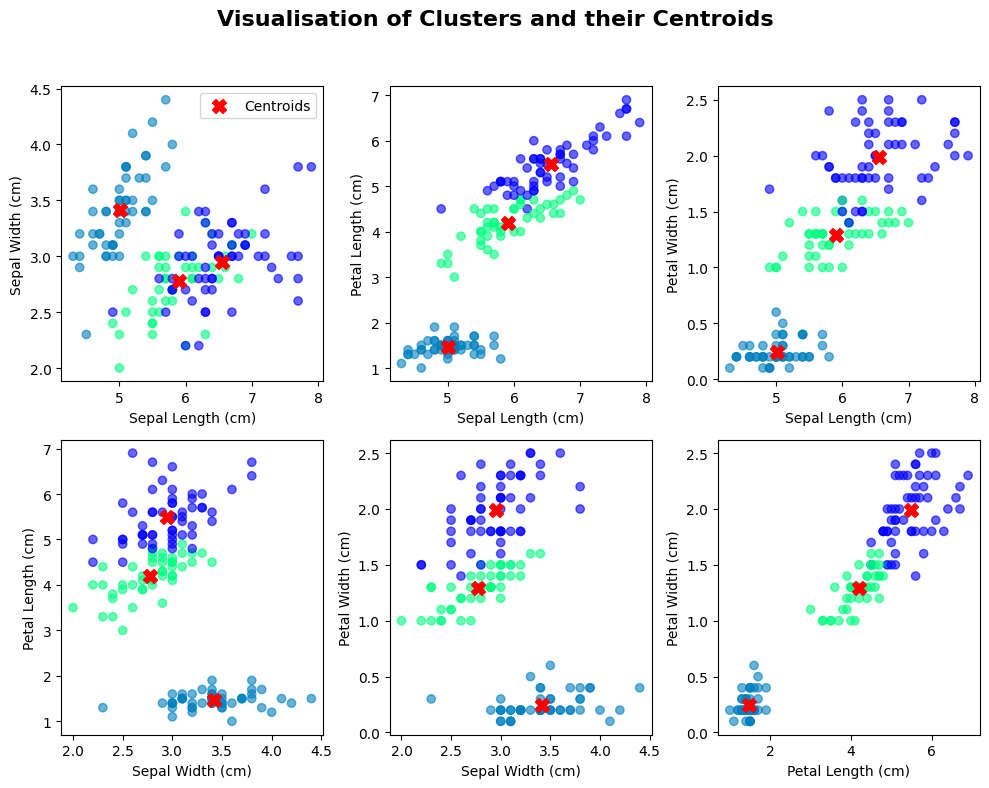
\includegraphics[width=\linewidth]{img/GM_iris.png}
    \caption{Gaussian Mixtures before CLL}
    \label{fig:iris_before}
  \end{minipage}\hfill
  \begin{minipage}{0.49\textwidth}
    \centering
    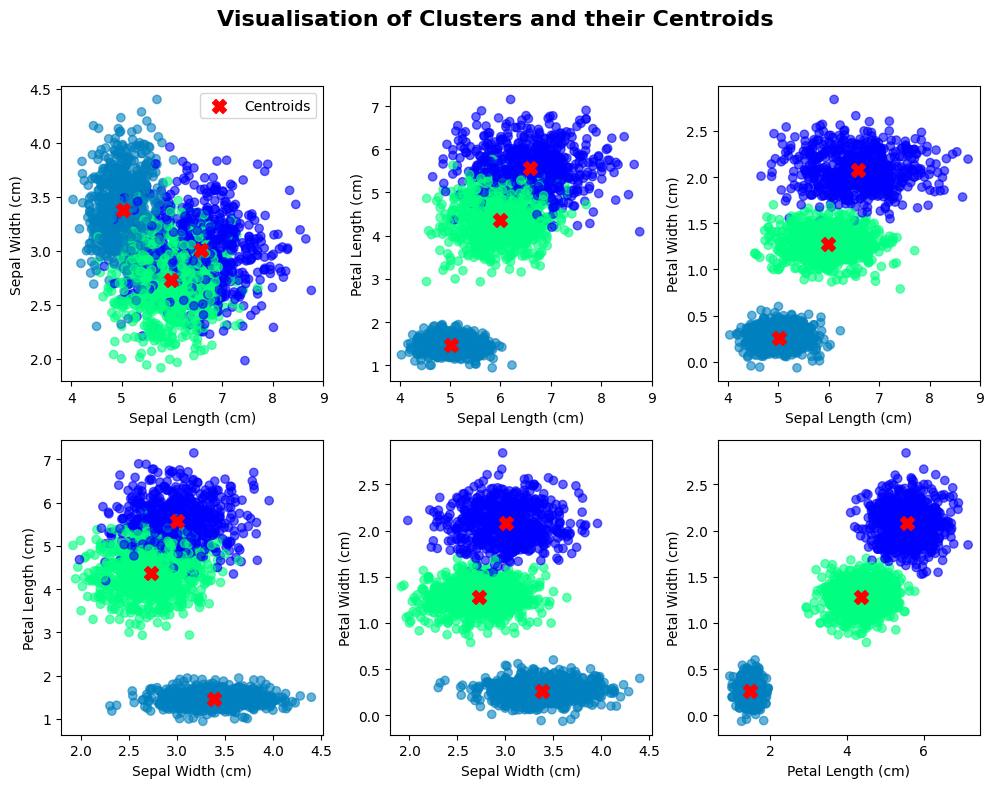
\includegraphics[width=\linewidth]{img/GM+CLL_iris.png}
    \caption{Gaussian Mistures after CLL (200 steps, $M=20$)}
    \label{fig:iris_after}
  \end{minipage}
\end{figure}

We get these displacements of the centroids at each step:

\begin{figure} [H]
    \centering
    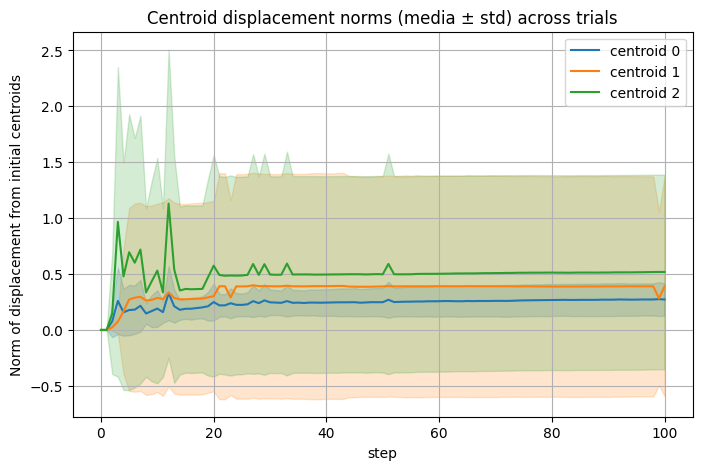
\includegraphics[width=\linewidth]{img/GM_displacement.png}
    \caption{Displacements of centroids with Gaussian Mixtures on Iris database}
\end{figure}
and we get a quality of:
\begin{equation*}
    Q=\frac{\frac{0.131}{3.15}+\frac{0.044}{3.19}+\frac{0.202}{2.38}}{3}=0.046
\end{equation*}
much worse than the quality of the KMeans clustering of Iris Database.